\chapter{Understanding phytoplankton community shifts in the eastern Cariaco basin}

\small {\textbf{This is the current state of progress towards the first manuscript}}


\normalsize
\section{Regime shift in the Cariaco Basin}
The CARIACO time-series has been collecting detailed data on the phytoplankton community in the Cariaco Basin from 1995 to 2017 (see Section \ref{CARIACOintro} for a full description). 
% this is repetitive
What has been a particular focus of the research based on this data set is the apparent changes in environmental conditions documented in both the physical boundary conditions as well as the biological data. \citet{Taylor2012} described a state shift in the biotic community. 
Using the fluorometric $chl~a$ data collected their analysis proposes a reduction in phytoplankton biomass, coinciding with a reduction in nutrient upwelling. % EST this sentence is unclear revise!
An increase in zooplankton abundances (although the measurements of this were only commenced in 2001) was linked to a collapse in sardine fisheries in the region (see Figure \ref{TaylorSHIFTS}). \citet{Pinckney2015} further expanded on this work by looking in detail at both the phytoplankton taxonomy data, as well as HPLC-derived $chl~a$ data. The HPLC-derived data showed no clear reduction in total $chl~a$ and spoke against a reduction in phytoplankton biomass. In comparison to the fluorometric method, HPLC can measure the concentrations of multiple pigment types and the total chlorophyll signal is less influenced by the specific pigment composition of the phytoplankton community. What the data showed specifically was that instead of a reduction in total chlorophyll within the water column, overall bloom intensity (i.e. the variability in biomass) decreased and phytoplankton moved to greater depth (see Figure \ref{TChlAPinckney}). This is also supported by irradiance measurements showing a reduction in the depth of the euphotic zone \citep{Pinckney2015}. Using the software CHEMTAX, the individual pigment composition can be used trace the proportion of total chlorophyll biomass that is substituted by the individual functional groups. 
% you dont have to keep repeting this so many times:
This data was kindly supplied by James Pinckney and forms the basis of the planned study.

\begin{figure}
\centering
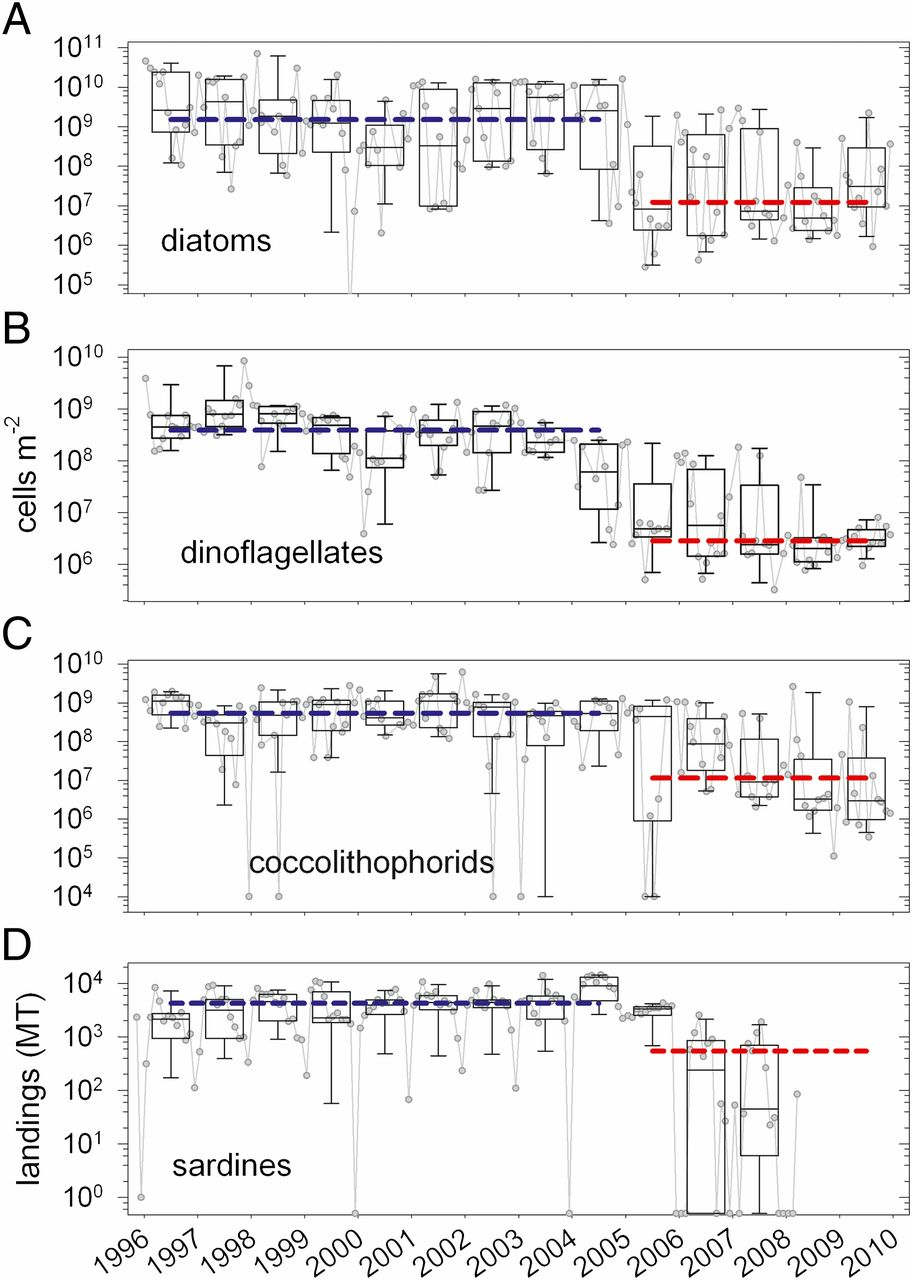
\includegraphics[trim = 0mm 0mm 0mm 0mm, clip, width=0.7\linewidth]{./Chp2-Pre/Tayloretal2012_F3.large.jpg}
\caption[Scheme]{\small {"Shifts in phytoplankton community composition and sardine landings from the southeastern Margarita Island fishery. Monthly observations presented as gray symbols. Box and whisker plots depict binned annual variations in diatom (A), dinoflagellate (B), coccolithophorid (C) inventories integrated over the upper 55 m and sardine fishery landings (D) in metric tons. Boxes represent the interquartile range of all observations (25th to 75th percentiles). Internal horizontal lines and whiskers are medians and 10th to 90th percentiles, respectively. Blue and red horizontal lines represent the grand medians of all observations between 1996 and 2004 and between 2005 and 2009, respectively. Data in early and late bins are significantly different in all cases (ANOVA; P \textless 0.001). [Fishery data are courtesy of L. W. Gonzáles (Universidad de Oriente, Boca de Río, Isla de Margarita, Venezuela); zero values artificially set at 0.5 for plotting purposes.)" from \citet{Taylor2012}}} % rewrite in own words, or use own plot!
\label{TaylorSHIFTS}
\end{figure}

\begin{figure}
\centering
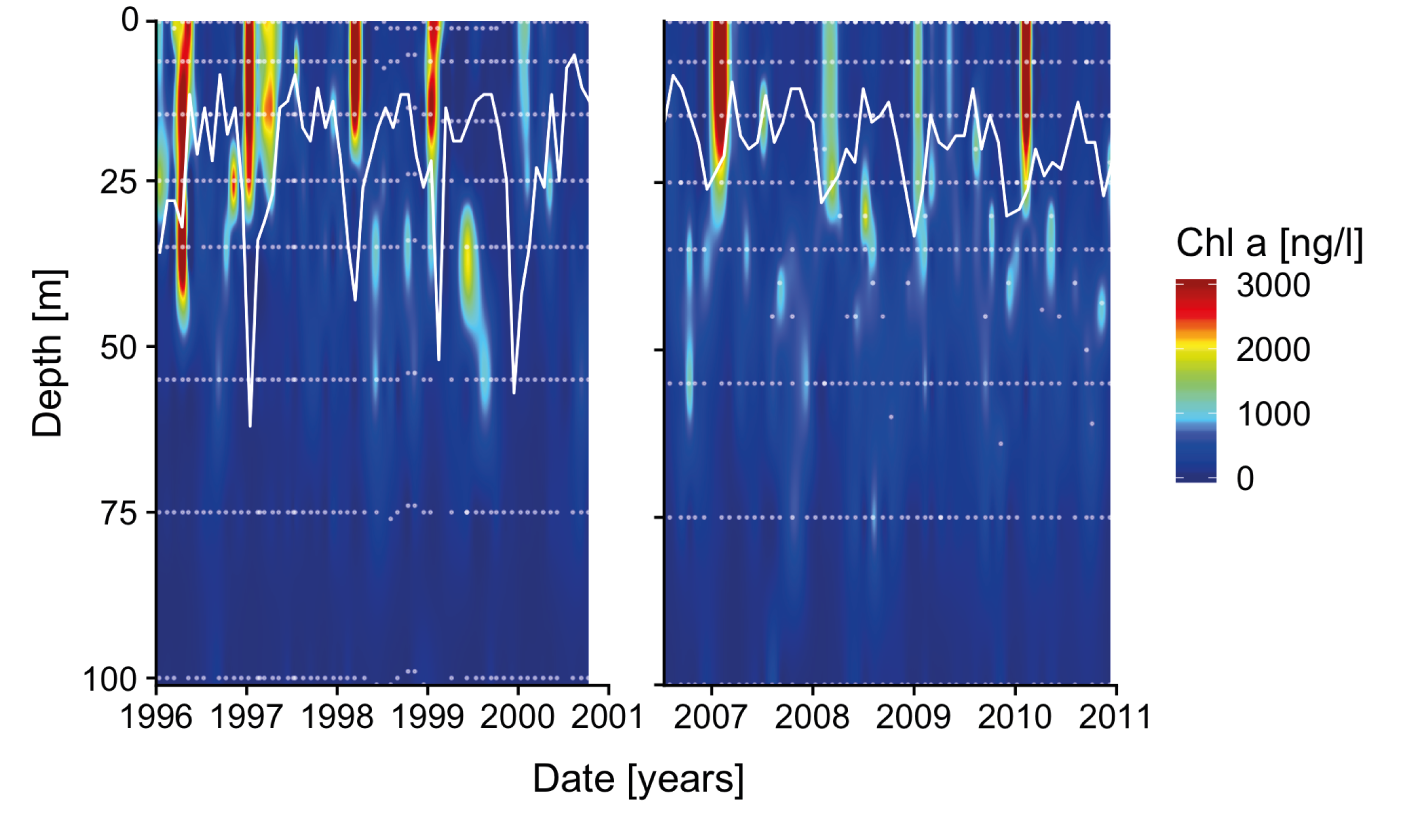
\includegraphics[trim = 0mm 0mm 0mm 0mm, clip, width=.9\linewidth]{./Chp2-Pre/Pinckneyetal2015_TotChlAcontoursMLD.png}
\caption[Scheme]{\small {Contour plot of HPLC-measured $chl~a$ for the two time periods with full data coverage (January 1996 to October 2000 and July 2006 to December 2010). Light white dots indicate data points. White line shows the depth of the mixed layer. HPLC Data and MLD depth was received from James Pinckney and Claudia Benitez-Nelson.}} % keep only one reference to data received
\label{TChlAPinckney}
\end{figure}


\begin{figure}
\centering
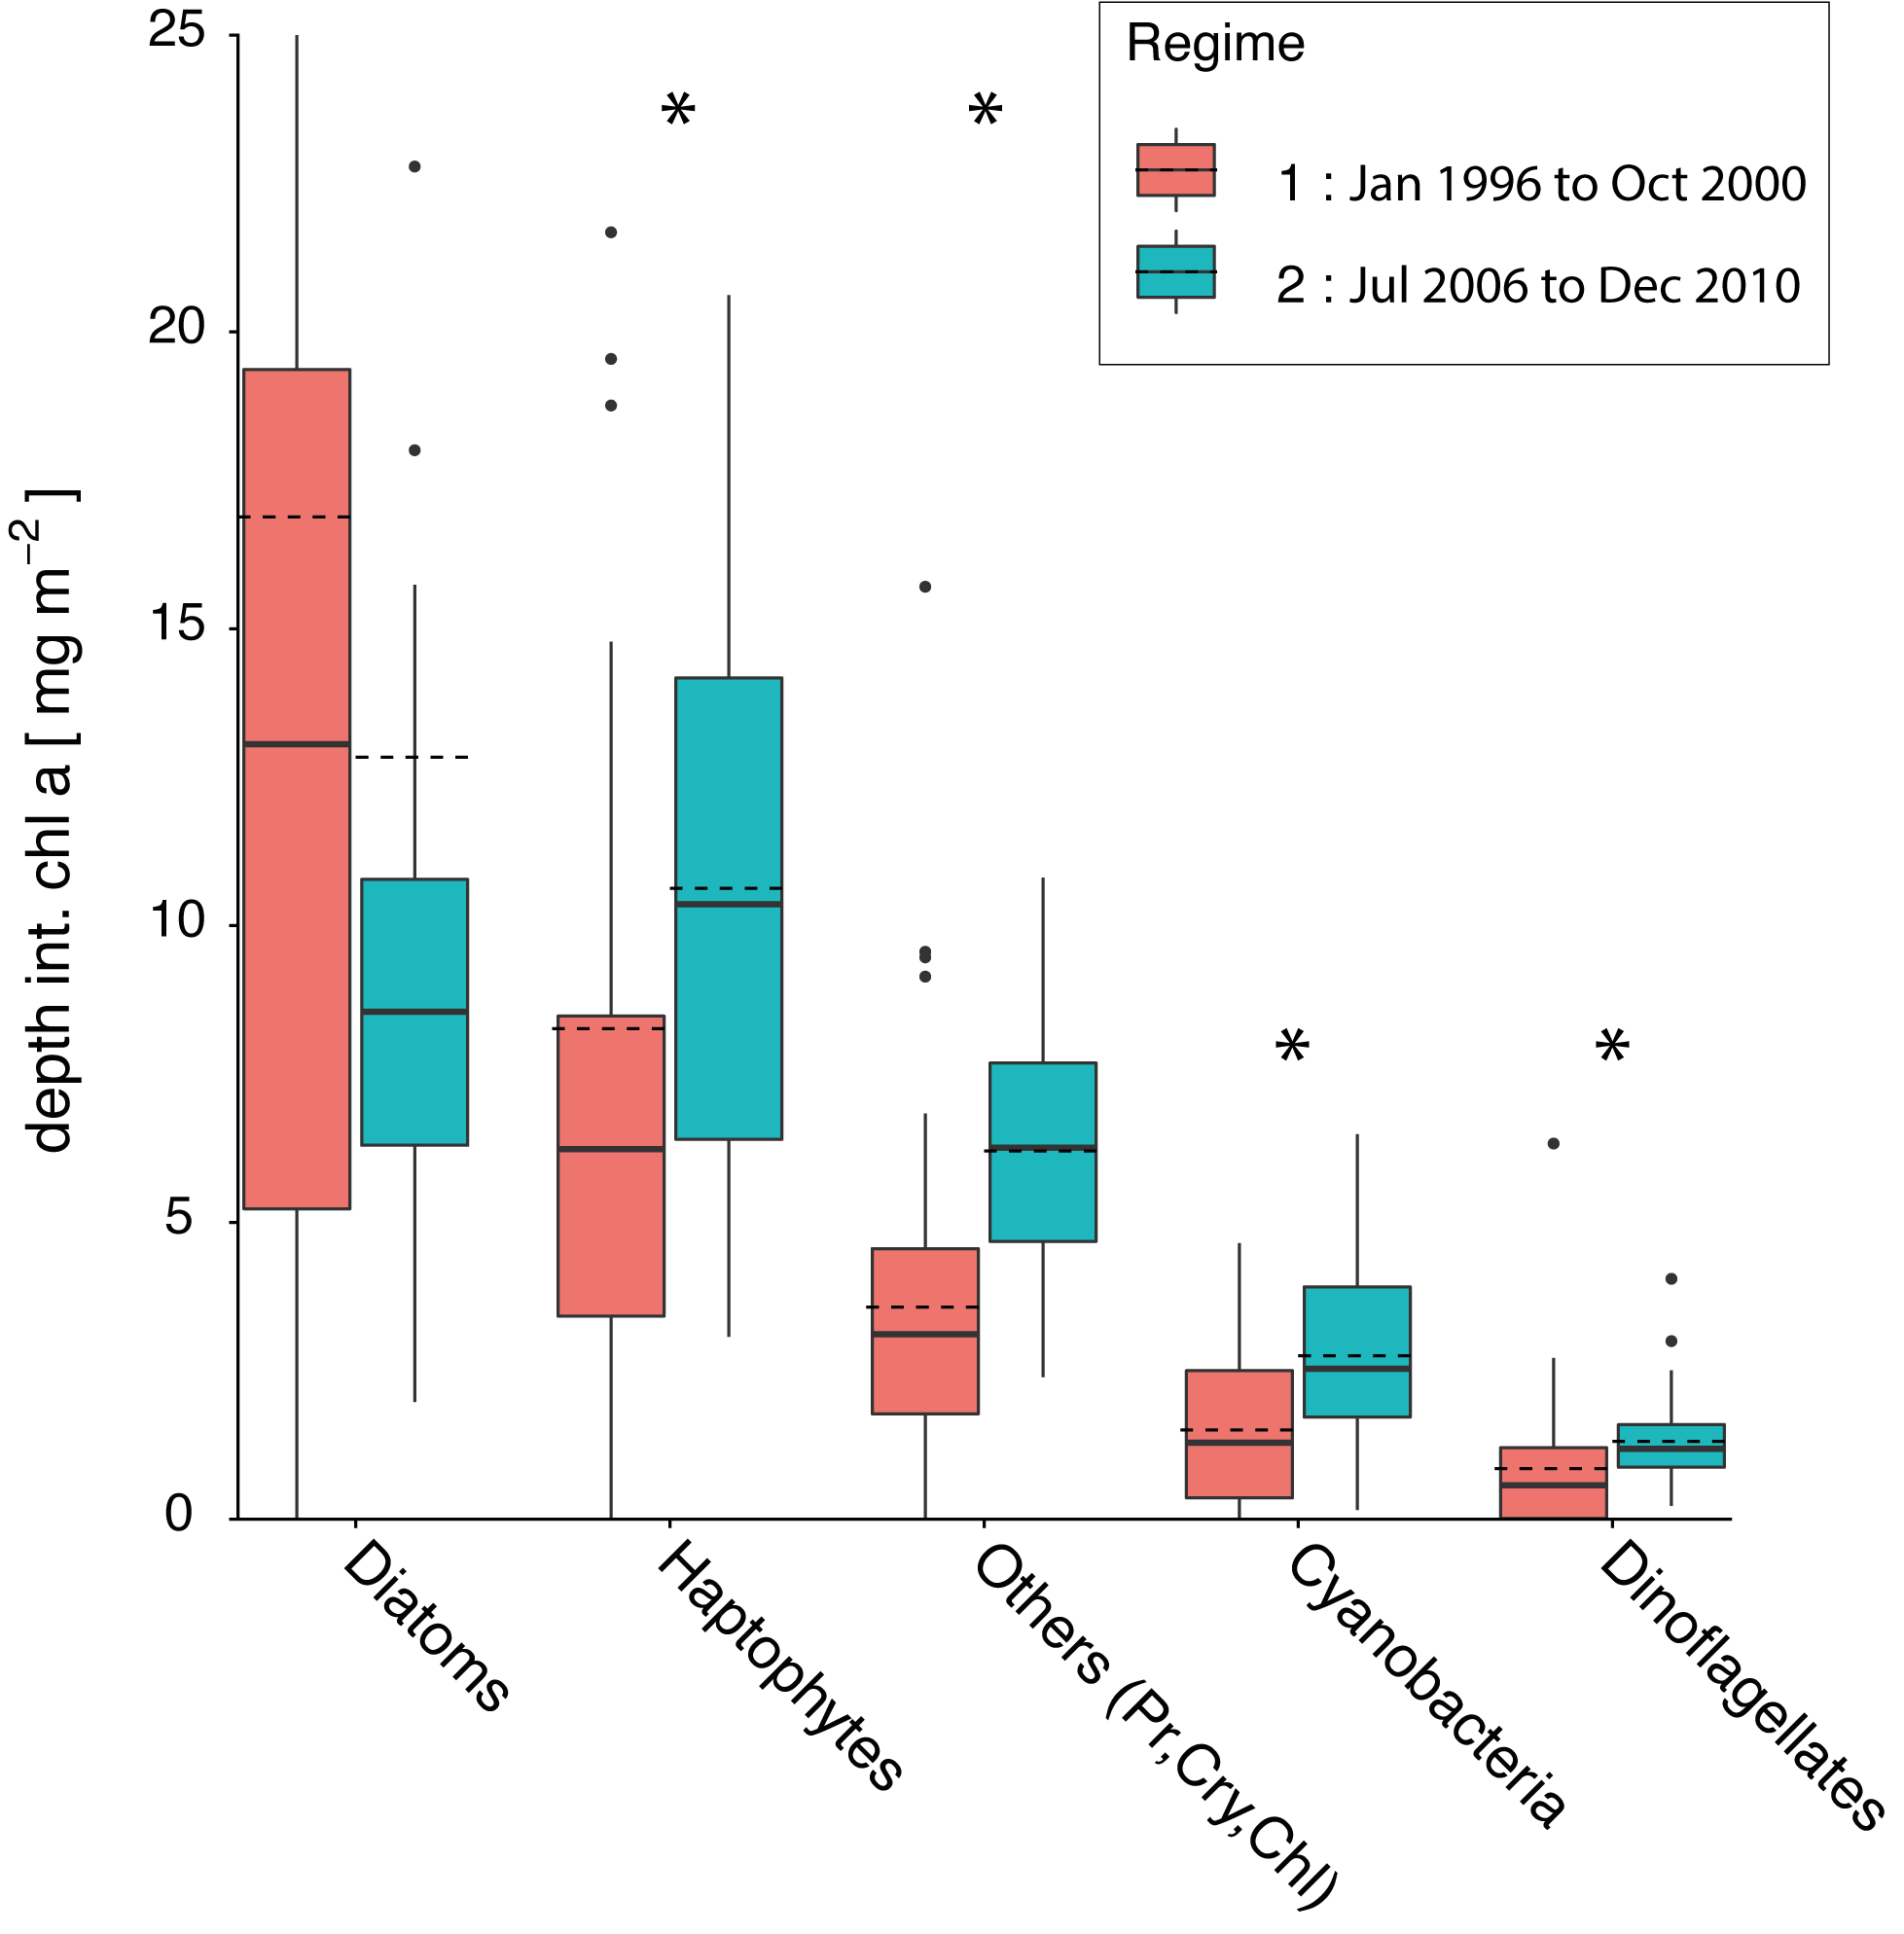
\includegraphics[trim = 0mm 0mm 0mm 0mm, clip, width=.7\linewidth]{./Chp2-Pre/PFT_groupsAsset511.png}
\caption[Scheme]{\small {Boxplots of HPLC-measured $chl~a$ depth integrated to 100 m for the two time periods with full data coverage. Boxplots illustrate the 25th and 75th quartiles (the box), the whiskers show the 5th and 95th percentiles, full line shows the median, dotted line shows the mean value per regime. Asterisk * indicates a significant difference between Regimes 1 and 2 in a one-sided t-test (p \textless	 0.05). 
% why a ttest  and did you carefully checked that you could preform the  with this data, i.e. that you follow all  the assumptions of the test?
Functional type $chl a$ was separated using the software Chemtax as described in \citet{Pinckney2015}}}
\label{PFTcariaco}
\end{figure}

\begin{figure}
\centering
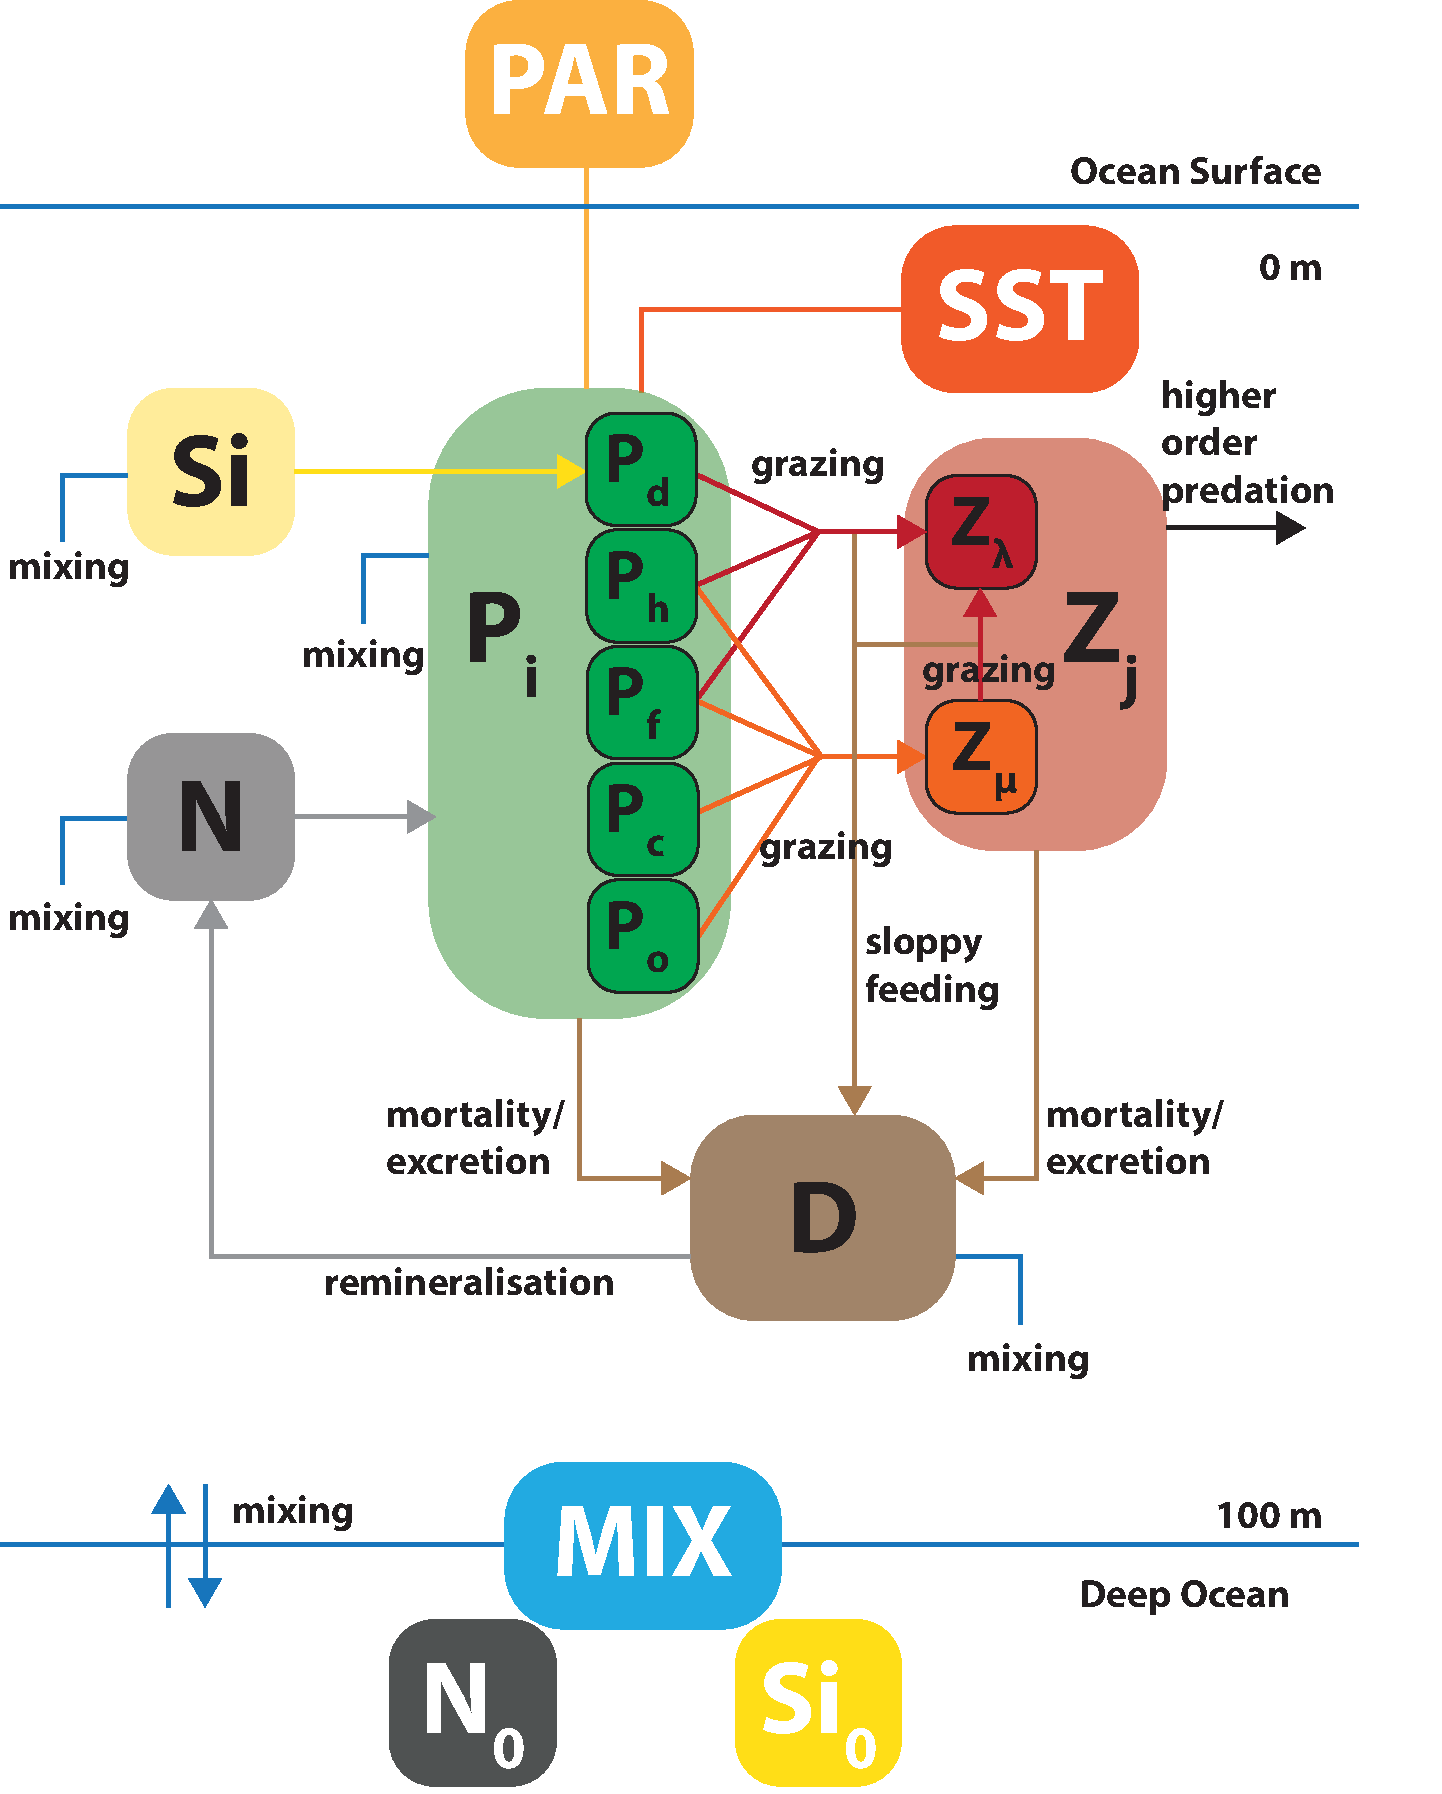
\includegraphics[trim = 0mm 0mm 0mm 0mm, clip, width=1.\linewidth]{./Chp2-Pre/ModelSchematicsAsset1111.pdf}
\caption[Scheme]{\small {Model schematics of current iteration of the ecosystem model.The ecosystem is embedded in a box of fixed depth. Nutrients below are assumed to be constant, mixing is a function MLD to simulate seasonal upwelling. See the methods description for a full explanation of model components.}}
\label{ModelSchematics}
\end{figure}


\begin{figure}
\centering
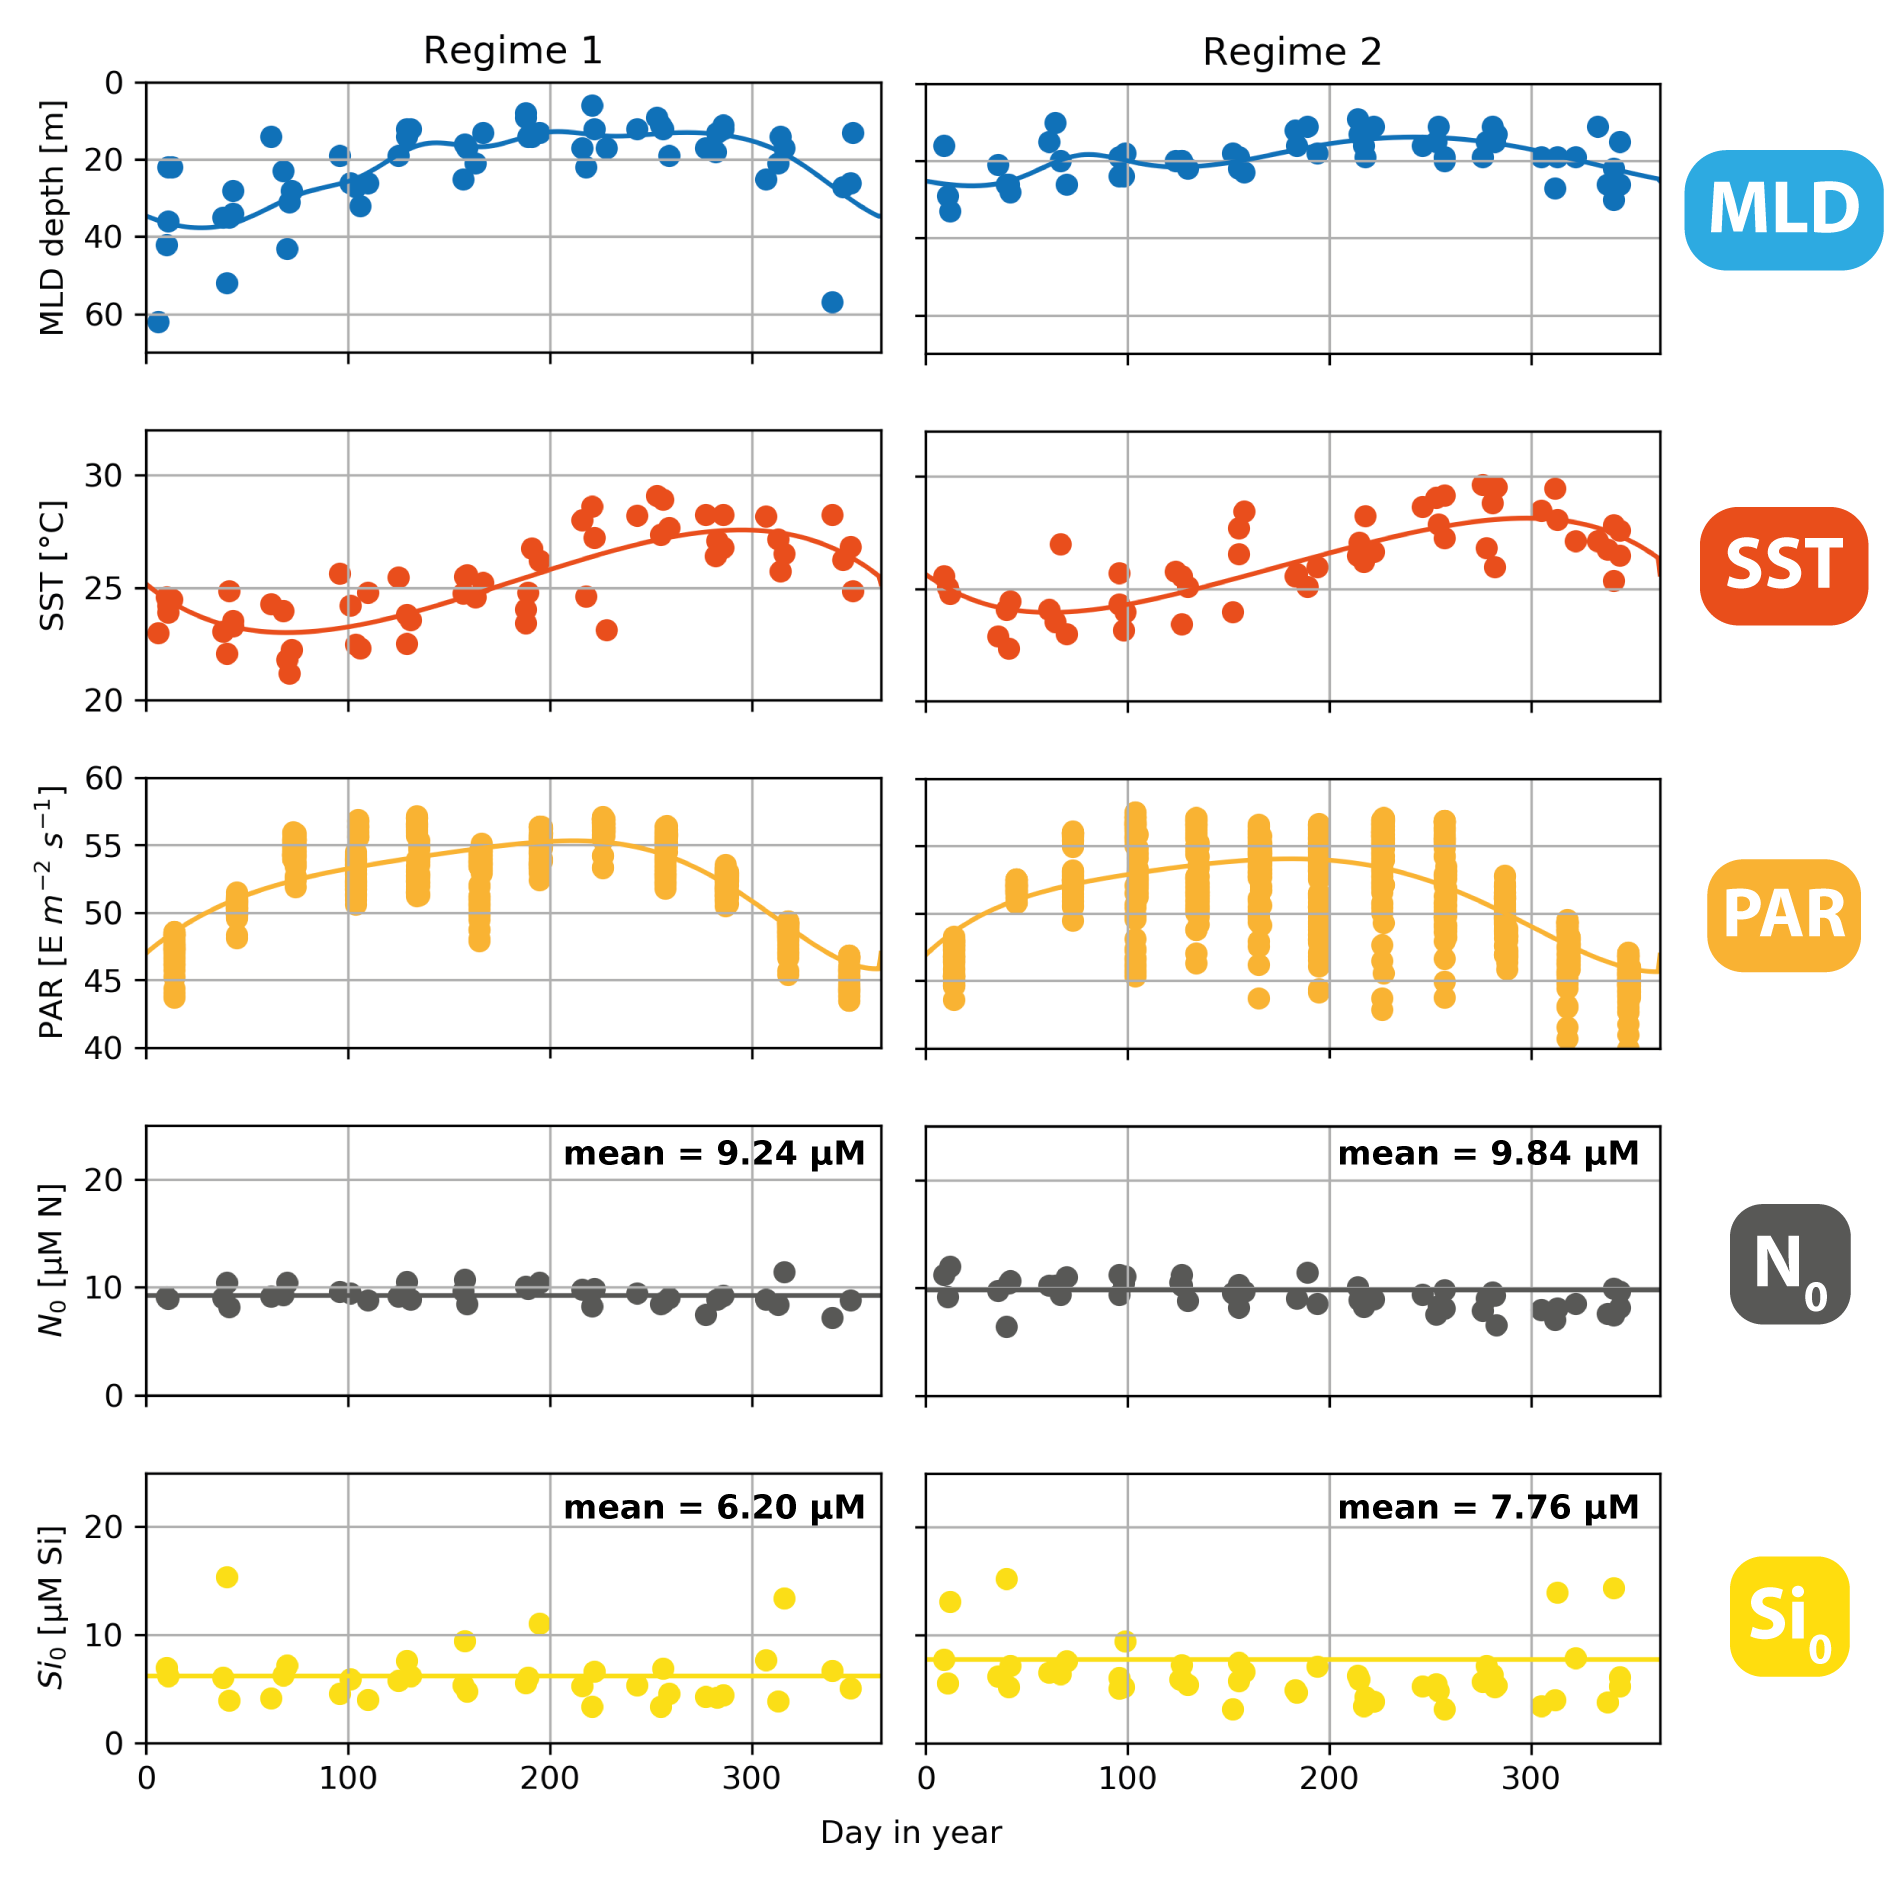
\includegraphics[trim = 0mm 0mm 0mm 0mm, clip, width=1.\linewidth]{./Chp2-Pre/ForcingAsset411.png}
\caption[Scheme]{\small {Aggregated forcing per the two regimes adapted from \citet{Pinckney2015}. Regime 1 from January 1996 to October 2000, Regime 2 from July 2006 to December 2010, values are aggregated to a single year. Depth profiles of Nitrate and Silicate were interpolated to depth and averaged between 100 and 150 m. Continous line shows interpolated values of MLD, PAR and SST used for model forcing and mean values for N and Si due to the assumption of a constant value at depth. SST and PAR data is taken from SeaWiFS satellite monthly climatological data. }}
\label{ModelForcing}
\end{figure}

The two regimes described by \citet{Pinckney2015} do not describe a formally analyzed time point, but rather are the two time periods were HPLC data coverage was given. The previous analysis by \citet{Taylor2012} places the changing point into the year 2005, which coincides with the time point right before the second time period where HPLC-data was continuously measured. 
% EST: could you point out to the figure where the reader can observe this?
The term regime shift is actually not very well defined and has been used uncritically in the scientific literature \citep{DeYoung2004a}. There are global trends and indications of a regime shift, but methods to identify regime shifts are not well established and have been critically discussed in the literature \citep{Steele2004a, Mantua2004a, Litzow2016a}. To my knowledge no formal exploration of a potential regime shift has been performed with the CARIACO data, therefore the term regime shift is used here to describe the observed changes in the phytoplankton community and physical environment without presupposing a formally defined state shift in the entire ecosystem. 
% first your started the paragraph from something specific about the cariaco regime shifts and now you move to a general aspects of regime shifts. This is a confusing structure for the paragraph please revise it and consider to develop each paragraph from the general to the specific
% EST: what is a state shift then? you also use uncritically not well defined terminology. You have to provide the reader with more context and define properly the terms, particularly does that form the basis of your work and that would lead to confusion 

The variability in environmental conditions in Cariaco between the two regimes can be seen in the aggregated model forcing
% EST: aggregate over what?
 (see Figure \ref{ModelForcing}).
% EST: figure 2.5 cited before figure 2.3 and 2.4 also, better arrange the figures so it the redear does not have to scroll down several pages in order to see what you are citing 
  There is a clear reduction in MLD variability, which allows me to use this as one of the drivers of a possible regime shift, however I plan on performing a more formal analysis of the regime forcing in the future. 
  % how? provide detail not just mention things
  The other main hypothesis 
  % how "the other hypothesis" is logically linked to the variability of environmental conditions? please revise the logic structure of the paragraphs and try to make your work more comprehensible
  that has been put forward as a possible explanation of the shifts in the phytoplankton community, in particular towards smaller sizes of phytoplankton, is the collapse in the sardine fisheries and the subsequent increase in zooplankton biomass. 

Although the zooplankton data does not cover the the first time-period of HPLC-data coverage, there measurements of the $Phaeo$ pigment over the entire time period. 
% what??? revise this whole paragraph
$Phaeo$ pigment is a results of chlorophyll degradation and can be used as a proxy for zooplankton grazing pressure. The overall dynamics point towards an increase in grazing pressure, coinciding with the increase in zooplankton abundance that was documented \citep{Pinckney2015}. In the model the collapse of the sardine fisheries, an important grazer of zooplankton, can be directly implemented through the higher-order mortality term acting on zooplankton (see Figure \ref{ModelSchematics}). 
% properly describe the model schematic not just mention it!

As there has to date been no ecosystem modeling study performed in the region,
% in the introduction you meintion there was one study!
I am using a relatively simple model formulation without an explicitly trait-based treatment of diversity.
% in the introduction you meintion there was one study!
Instead I focus on resolving the phytoplankton and zooplankton functional types that were directly measured in the time-series. For phytoplankton, the data used is the functional-type resolved HPLC-derived $chl~a$ data presented by \citet{Pinckney2015}.
% EST: this is cumbersome 
 The CHEMTAX analysis resolved 7 functional types in total, based on the pigments that were measured. To simplify the implementation and parametrization of the model, these were aggregated to 5 groups as presented in Figure \ref{PFTcariaco}. 
 % EST: describe figure properly, what do you see? and quoting order should correspond to number, 2.3 after 2.4 right now!
 As the groups of Cryptophytes, Prasinophytes and Chlorophytes do not present a unique biogeochemical role and showed similar dynamics, they were aggregated to the "Others" group. This is a preliminary grouping for initial analysis. Zooplankton were measured using bongo net tows with two different mesh sizes of 200 and 500 microns. The model resolves these as two separate zooplankton types.





\section{Methods}
% EST: The description of the data and the study site it is more appropriately located in the Material & Methods section

{\bf {Model description}} 

NPZD models are simplified marine ecosystem models
% what am i trying to say here?
 that can be adapted to different physical settings and food web structures. For this model, the basic ecosystem structure is inspired by the models of Fasham (1990). The physical setting of the model uses a zero-dimensional structure where a fixed volume of water resides above a deep homogenous layer. The code structure is the PhytoMFTM model (as explained in Section 3)
 % EST: is should be explained first
 written in the open source programming language Python, which provides a flexible framework for NPZD-type models with multiple functional types of phytoplankton and zooplankton. The model code and all statistical scripts are available publicly on Github (\url{https://github.com/ben1post/BennyPhD}).

The model framework was adapted to the setting of the CARIACO time-series in the Cariaco basin of the coast of Venezuela. The data includes phytoplankton functional-type resolved HPLC data 
% EST: is should be explained first
and two size-classes of zooplankton, which were included in the model as the 5 phytoplankton types, and 2 zooplankton types. The phytoplankton types include Diatoms $P_{d}$, Haptophytes $P_{h}$, Dinoflagellates $P_{f}$, Cyanobacteria $P_{c}$ and Others (representing a generalized small green algae) $P_{o}$. There are two Zooplankton types split by size class, named Mikrozooplankton $Z_{\mu}$ and Mesozooplankton $Z_{\lambda}$. 

Nitrogen $N$ (and Silicate $Si$ for Diatoms) is assimilated by the phytoplankton types $P_i$, which are grazed by the zooplankton types $Z_j$. Mortality of and excretion from phytoplankton and zooplankton, and sloppy feeding by zooplankton contribute to Detritus $D$. In addition to the linear mortality of $P_i$ and $Z_j$, there is an additional quadratic mortality term acting on $Z_j$, which represents higher-order predation on zooplankton. Other nutrients are not implemented yet, but might be as the work progresses. The functional types 
% EST: WHICH FUNCTIONAL TYPES?
differ only in their nutrient uptake dynamics and growth rates.
% EST: HOW SO?
 Nitrogen-fixation of Cyanobacteria, which has been documented in the Cariaco Basin \citep{Montes2013}, could also be explicitly included, but has not been to date. 
 % EST: consider to avoid to mentions details that are irrelevant to the interpreation of current results

{\textbf{Model physics in a tropical coastal setting}}

The ecosystem component of the model is set within a zero-dimensional physical environment. The water column is divided into a box of 100 meters depth, above a homogenous deep layer. 
% EST: repetitive
There is no lateral advection, but vertical mixing is modeled as a function of mixed layer depth (MLD) over time $M(t)$. Temperature depth profiles have been used to reconstruct the MLD at the investigated location. 
The derivative of MLD over time is given as $h(t) = dM(t)$. 
% EST: this comes out the blue to what is related at this point?
Exchange between the two layers is described by the two processes of turbulent diffusion and upwelling, 
% EST: how?
with the depth of the MLD as a proxy for the strength of exchange between the two layers. The effects of entrainment and detrainment on nutrients, are given by the term $h^{+}(t)= max[h(t),0]$. 
% EST: i found this description very confusing and would be able to reproduce what you did, please consider to rewrite it
Phytoplankton and detritus are assigned a constant sinking rate as of now, but this could be also be modified as a function of MLD depth. Zooplankton is assumed to be able to maintain themselves within the model boy,
% MODEL BOX
therefore $Z_j$ is not modified by the upwelling term. Diffusive mixing between the layers has been parameterized with a constant factor $k$. The entire upwelling term is thus
\begin{equation}
\kappa = \frac{k + h^{+}(t)}{M(t)}
\end{equation}
% this is basically Evans and Parslow formaulation like Fasham used in 1990? why you explained it so complicated? and why you did not cite them?
In addition to the MLD interpolated from time series data, the model is externally forced with sea surface temperature (SST) and interpolated from monthly to daily values and photosynthetically active radiation (PAR) from monthly averaged SeaWIFs satellite data.
% EST: above unclear, revise! 
This model construct is a preliminary modification of the typical slab model, as described in \citet{Anderson2015}. A slab model describes the ecosystem component above a variable MLD, however this is not suitable in the tropical coastal location of the Cariaco Basin, as exemplified in Figure \ref{BelowMLD}. Since the MLD is much shallower than in temperate settings, there is no constant nutrient concentration below the MLD, instead it is highly variable. In addition to this, in a typical slab model phytoplankton below the MLD is not described. In temperate settings the MLD can reach far below 100m and thereby far below the euphotic zone. In Cariaco the MLD is generally above the euphotic zone and there is a considerable concentration of phytoplankton growing below the MLD. Therefore the box model structure, resolving the top 100 m was adopted.
% why mention this here and not from the beginning where you describe the MLD, this is very confusing!


\begin{figure}
\centering
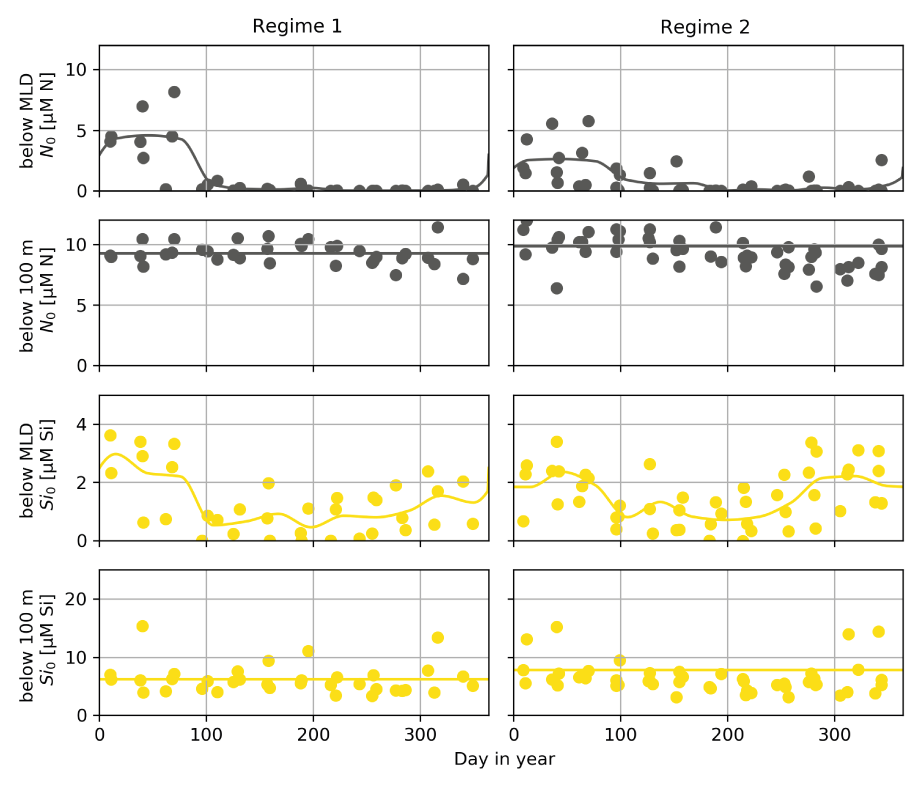
\includegraphics[trim = 0mm 0mm 0mm 0mm, clip, width=0.68\linewidth]{./Chp2-Pre/NutsBELOWmldAsset1011.png}
\caption[Scheme]{\small {Nutrient concentrations below MLD and averaged between 100 and 150 m depth for both regimes aggregated to one year. For values below MLD the continuous line represents interpolated forcing, for values below 100 m the line shows the mean value.}}
\label{BelowMLD}
\end{figure}



{\bf {Phytoplankton}}

Phytoplankton growth is a function of light (PAR), temperature (SST) and nutrients.
% WHICH NUTRIENTS?
 These factors are assumed to independently limit growth, so that (exemplary for $P_{d}$, i.e. diatoms) the growth term is
\begin{equation}
\mu_{d} = \mu_{d}^{max} \cdot U_{d}(N,Si)\cdot L_{d}(PAR)\cdot T_{d}(SST)
\end{equation}
where $\mu_{d}^{max}$ is the maximum growth rate per day and $T(PAR)$ is Eppleys formulation for temperature dependent growth, given as $T(SST) = e^{0.063 * SST}$ with temperature in $^\circ C$. The light-limiting term $L(PAR)$ represents the integrated photosynthesis within the mixed layer as a function of incident irradiance at the surface $I_0$. Light attenuation is calculated using the Lambert-Beer law with irradiance at depth $z$ equal to
\begin{equation}
I(z) = I_0 \cdot e^{-k_{PAR} \cdot z}
\end{equation}
Here, $k_{PAR}$ is calculated as the sum of the constant attenuation coefficient of water $k_w$ and the self-shading of phytoplankton $k_c$ with the unit $\mu M^{-1}$ multiplied by total phytoplankton biomass $P$, i.e. $k_{PAR} = k_w + k_c P$. This model uses the Smith PI curve as a basis for the calculation, with $V_P$ representing the photosynthetic rate, $\alpha$, the initial slope of the PI curve and $V_p^{Max}$, the maximum photosynthetic rate
\begin{equation}
V_p = \frac{\alpha \cdot I \cdot V_p^{Max}} {\sqrt{(V_p^{Max})^2 + \alpha^2 \cdot I^2}}
\end{equation}
Combining equation (2) and (3) as presented in \cite{Anderson2015}, the integrated photosynthesis $\bar{V}_p$ over depth $z$ is calculated as
% EST: the bar above is the letter is not the right symbol for integration  please correct this... ME: rly though?
\begin{equation}
\bar{V}_p(z) = \frac{V_p^{Max}}{k_{PAR} \cdot z} \cdot \ln \Bigg( \frac{\alpha \cdot I_0 + \sqrt{(V_p^{Max})^2+(\alpha \cdot I_0)^2}} {\alpha \cdot I(z) + \sqrt{(V_p^{Max})^2+(\alpha \cdot I(z))^2}} \Bigg)
\end{equation}
where $\bar{V}_p$ equals the light-limiting term $L$ in the growth equation (2).
% explain all params in eq!

Nutrient limited growth of the phytoplankton community is described via a Monod equation. 
\begin{equation}
U(N) = \frac{N} {k_N + N}
\end{equation}
% explain all params, what is k_N? 
For diatoms $P_d$ the nutrient limiting term depends on both nitrogen and silicate concentration within the upper layer. According to Liebig's law of the minimum, always the lower nutrient availability limits Diatom growth:
\begin{equation}
U_{d}(N,Si) = min \Big( \frac{N} {k_{d}^N + N}, \frac{Si} {k_{d}^{Si} + Si} \Big)
\end{equation}
All other phytoplankton types are nutrient-limited only by available Nitrogen as in equation (6). Phytoplankton mortality and excretion are parameterized as a linear constant rate $mo$. 
% EST: only use single letters for parameters
Phytoplankton sinking is defined by the parameter $v$.With $G_{\mu}$ as grazing by Microzooplankton and $G_{\lambda}$ as grazing by Mesozooplankton (defined below), the equations for all phytoplankton types $P_i$ can be written as
\begin{equation}
\frac{dP_{i}}{dt} = \mu_{i} \cdot P_{i} - mo_{i} \cdot P - G_{\mu}(P_{i}) - G_{\lambda}(P_{i}) - v \cdot P_{i}
\end{equation}

{\bf {Zooplankton}}

Two zooplankton types are Microzooplankton $Z_{\mu}$ and Mesozooplankton $Z_{\lambda}$. Following Anderson et al. (2015) the grazing of, for example, $Z_{\lambda}$ on diatoms $P_d$ is formulated as follows

\begin{equation}
G_{\lambda}(P_{d}) = \Bigg( \frac{\mu^Z_{\lambda} \cdot \phi^{\lambda}_d \cdot P_d} 
							{(k^Z_{\lambda})^2 + \phi^{\lambda}_d \cdot P_d + \phi^{\lambda}_c \cdot P_c + \phi^{\lambda}_{df} \cdot P_{df} + \phi^{\lambda}_{n} \cdot P_{n} + \phi^{\lambda}_{\mu} \cdot Z_{\mu}} \Bigg) \cdot Z_{\lambda}
\end{equation}
$\phi^{\lambda}_{d}$ = $\rho^{\lambda}_{d} P_{d}$ , $\phi^{\lambda}_{c}$ = $\rho^{\lambda}_{c} P_{c}$ , $\phi^{\lambda}_{df}$ = $\rho^{\lambda}_{df} P_{df}$ , $\phi^{\lambda}_{n}$ = $\rho^{\lambda}_{n} P_{n}$ , $\phi^{\lambda}_{\mu}$ = $\rho^{\lambda}_{\mu} Z_{\mu}$

with $\mu^Z_{\lambda}$ as the maximum grazing rate, $k^Z_{\lambda}$ as the half saturation constant of grazing, $\phi^{\lambda}_{d}$ as the density dependent feeding preference of $Z_{\lambda}$ feeding on $P_d$, defined as $\rho_{d} \cdot P_{d}$, with $\rho^{\lambda}_{d}$ as the feeding preference coefficient.


% EST: what about the other state variables Nutrient and detritus and the processes that control their fluxes?


{\bf {Solving method}}

The system of differential equations was solved numerically using the fourth-order Runge-Kutta method in the odeint function of the scipy package in python 3.7. 



{\bf {Full System of equations}}
% EST: There are several inconsistencies in the system of equations and the the equations presented before e.g. compared phytoplankton and zooplankton equantions
\begin{eqnarray*}
\frac{\partial N}{\partial t} & = & 
\kappa \cdot \left(N_{0} - N\right) + 
\delta^{N}_{D} \cdot D -
\sum_{i=1}^{n_P} [\mu_i \cdot U_{i}(N_0,Si_0)\cdot L_i(PAR)\cdot T_i(SST) \cdot P_{i}] 
\nonumber \\
\frac{\partial Si}{\partial t} & = & 
\kappa \cdot \left(Si_{0} - Si\right) 
- \mu_{dt} \cdot U_{dt}(N_0,Si_0) \cdot L_{dt}(PAR)\cdot T_{dt}(SST) \cdot P_{dt}
\nonumber \\
\frac{\partial P_{i}}{\partial t} & = & 
\mu_{i} \cdot U_{i}(N_0,Si_0)\cdot L_{i}(PAR)\cdot T_{i}(SST) \cdot P_{i}
- m_{i} \cdot P_{i} \\
&& - \sum_{j=1}^{n_Z} [I^{tot}_j \frac{p^i_{j} \cdot P_{i}} {R_{j}} Z_{j}] -
v\cdot P_{i} 
\nonumber \\
\frac{\partial Z_{\mu}}{\partial t} & = & 
\delta_Z \cdot I^{tot}_{\mu} \cdot Z_{\mu}-
\mu^{}_{\lambda} \frac{Z_{\mu}}{Z_{\mu}+k_{\lambda}} Z_{\lambda}-
m_{\mu} \cdot Z_{\mu} - 
g_{\mu} \cdot Z_{\mu}^{2}
\nonumber \\
\frac{\partial Z_{\lambda}}{\partial t} & = & 
\delta_Z \cdot I^{tot}_{\lambda} \cdot Z_{\lambda}+
\delta_{\lambda} \cdot \mu^{}_{\lambda} \frac{Z_{\mu}}{Z_{\mu}+k_{\lambda}} Z_{\lambda}-
m_{\lambda} \cdot Z_{\lambda} - 
g_{\lambda} \cdot Z_{\lambda}^{2}
\nonumber \\
\frac{\partial D}{\partial t} & = & 
\sum_{j=1}^{n_Z} [(1-\delta_Z) I^{tot}_j \cdot Z_{j}] +
(1-\delta_{\lambda}) \cdot \mu^{}_{\lambda} \frac{Z_{\mu}}{Z_{\mu}+k_{\lambda}} Z_{\lambda} \\
&& -\sum_{j=1}^{n_Z} [m_j \cdot Z_{j}] +
\sum_{i=1}^{n_P} [m_i \cdot P_{i}] -
v_{D} \cdot D -
\delta^{N}_{D} \cdot D
\nonumber
\end{eqnarray*}
 
where:\\
\mbox{} \hspace{0 cm} $N_0=$ Nitrogen concentration right below mixed layer [$\mu M$],\\
\mbox{} \hspace{0 cm} $N=$ Nitrogen concentration above mixed layer [$\mu M$],\\
\mbox{} \hspace{0 cm} $v=$ sinking rate of $P_i$ [$m$ $day^{-1}$],\\
\mbox{} \hspace{0 cm} $M(t)=$ mixed layer depth at time point $t$ [$m$],\\
\mbox{} \hspace{0 cm} $\kappa = \frac{1}{M(t)} \cdot \left(h^{+}(t) + \kappa\right)$ Constant that parameterizes diffusive mixing, \\
\mbox{} \hspace{0 cm} $h^{+}(t) = \max\left(0, \frac{d}{d t} M(t)\right)$ Function that describes upwelling as function of MLD,\\
\mbox{} \hspace{0 cm} $\delta^N_D=$ Remineralization rate of nitrogen component of detritus $D$ [$\mu M d^{-1}$],\\
\mbox{} \hspace{0 cm} $v_D=$ sinking rate of $D$ [$m$ $day^{-1}$],\\
\mbox{} \hspace{0 cm} $\mu_i=$Growth rate of phytoplankton type $i$ [$d^{-1}$],\\
\noindent
\mbox{} \hspace{0 cm} $U_i=\begin{cases}\min\left(\frac{N}{N + U^{N}_i}, \frac{Si}{Si + U^{Si}_i}\right),& \text{if P-type is Diatom}\\\frac{N}{N + U^{N}_i}, & \text{otherwise}\end{cases}$ Nutrient uptake of $P_i$,\\
\noindent
\mbox{} \hspace{0 cm} $L_i=\frac{1}{M(t) \cdot k_{w}} \cdot \left(e^{1 - \frac{PAR(t)}{Opt^{I}_i}} + e^{1 - \frac{PAR(t)}{Opt^{I}_i} \cdot e^{- M(t) \cdot k_{w}}}\right)$ Light dependence of  $P_i$,\\
\mbox{} \hspace{0 cm} $T_i= e^{0.063 \cdot SST}$ Temperature dependence of $P_i$,\\

\noindent
\mbox{} \hspace{0 cm} $P_i=$ Biomass of phytoplankton type $i$ [$\mu M N$],\\
\mbox{} \hspace{0 cm} $m_i=$ Mortality/excretion rate for phytoplankton type $i$,\\
\noindent
\mbox{} \hspace{0 cm} $I^{tot}_j= \mu^{Z}_j \cdot \frac{R_{j}}{R_{j} + k^Z_j}$ Total intake of zooplankton type $j$,\\
\mbox{} \hspace{0 cm} $k^Z_j =$ Half saturation constant of zooplankton type $j$,\\
\mbox{} \hspace{0 cm} $R_{j}= \sum_{i} (p_{i j} \cdot P_{i})$ Total ressource density of zooplankton type $j$,\\
\mbox{} \hspace{0 cm} $p^i_{j}=$ Feeding preference of zooplankton type $j$ feeding on phytoplankton type $i$,\\
\mbox{} \hspace{0 cm} $R_{\mu}= p^n_{\mu} \cdot P_{n} + p^{dn}_{\mu} \cdot P_{dn} + p^c_{\mu} \cdot P_{c}$ Total ressource density of Mikrozooplankton $Z_{\mu}$,\\
\mbox{} \hspace{0 cm} $R_{\lambda}= p^{dt}_{\lambda} \cdot P_{dt} + p^{dn}_{\lambda} \cdot P_{dn} + p^c_{\lambda} \cdot P_{c}$ Total ressource density of Mesozooplankton $Z_{\lambda}$,\\


\noindent
\mbox{} \hspace{0 cm} $Z_j=$ Biomass of zooplankton type $j$ [$\mu M N$],\\
\mbox{} \hspace{0 cm} $\delta_{Z}=$ Grazing efficiency of zooplankton on phytoplankton (represents sloppy feeding), \\
\mbox{} \hspace{0 cm} $g_{i}=$ Higher order predation on zooplankton (quadratic), \\
\mbox{} \hspace{0 cm} $m_{j}=$ Mortality/excretion rate for zooplankton type $j$,\\

\section{Preliminary Results}

The model as described is up and running, preliminary results are shown in Figure \ref{PrelimRes}. 
% EST: this is irrelevant!
As these are the results of using a parameter fitting routine implemented in the PhytoMFTM framework, the results are yet not entirely reasonable. One zooplankton type dominates, whilst the other is outcompeted. However the model is able to roughly recreate the nutrient dynamics observed in the first regime. The regimes are as defined by the HPLC data coverage, and the first regime will be used to create a baseline run to test the hypotheses on.
% EST: this is unclear
 Upwelling of nutrients can be modeled using the MLD forcing of the second regime and the collapse in sardine fisheries can be approximated with a reduction in the higher-order mortality term of zooplankton. 
 %  the hypothesis should be explained earlier not at this point 
 As the model physics are not yet settled, this will have an effect on the observed dynamics and comprehensive parameter fitting will be performed later on. 
 % but you define already how the "physics" of your model will be, why mentioning this here, does it add any crucial information to interpret your results? 

\begin{figure}
\centering
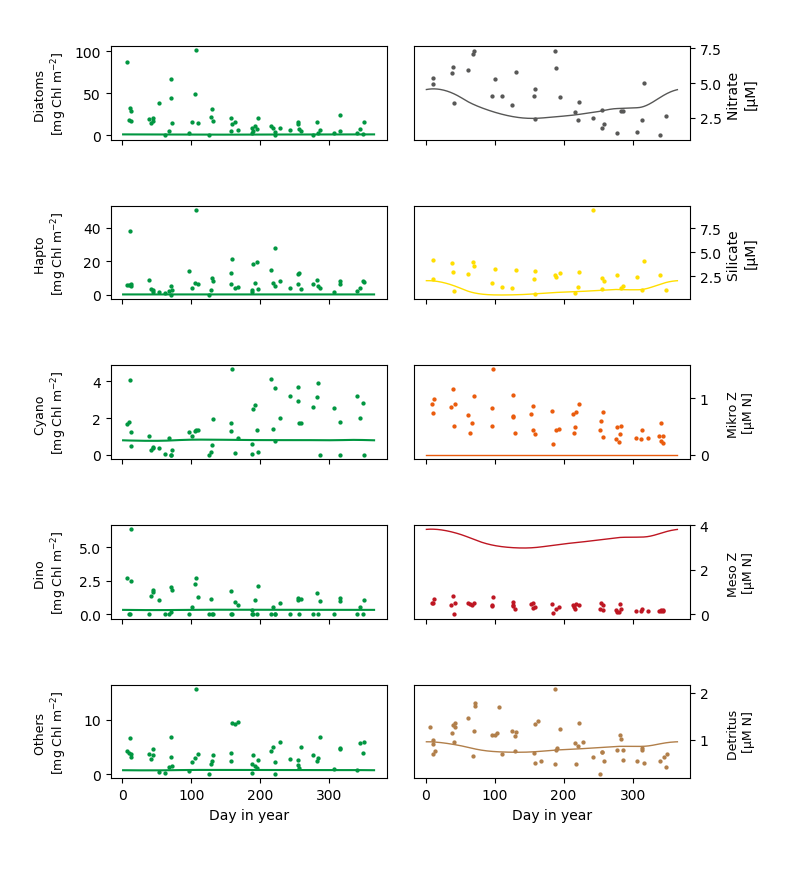
\includegraphics[trim = 0mm 0mm 0mm 0mm, clip, width=1.\linewidth]{./Chp2-Pre/Figure_1.png}
\caption[Scheme]{\small {Current best fit of preliminary model. Data is shown as dots, model results by continuous line. Model output is in units of $\mu M$ converted to integrated chlorophyll to compare to depth-integrated PFT $chl a$ pigment data.  Nutrient and detritus data was measured in $\mu M$. Zooplankton dry weight is converted by a carbon content of 32\% and a constant C:N ratio of 5.625. Clearly the model parameters are not ideal yet, however a general agreement with the PFT data and nutrient dynamics can be observed. Zooplankton parameters need to be adjusted to allow for a more realistic response.}}
\label{PrelimRes}
\end{figure}





